\documentclass{standalone}

\usepackage{circuitikz}

\begin{document}
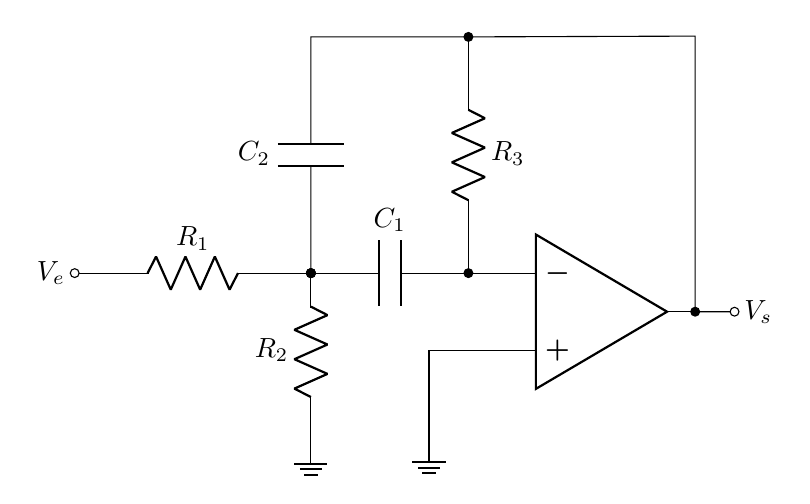
\begin{tikzpicture}
	\node[op amp, yscale=1] (opamp) at (6,-0.5) {};
	\draw ($(opamp.-)+(-5.5,0)$) node[left] {$V_{e}$} 
	to[R, l=$R_1$, o-*] ($(opamp.-)+(-2.5,0)$) node (nodebetween1) {}
	to[C, l=$C_1$, *-*] ($(opamp.-)+(-0.5,0)$) node (nodebetween2) {}
	to[short] (opamp.-);
	\draw (nodebetween1.center) to[R, l_=$R_2$, *-] ($(nodebetween1)+(0,-2)$) node [ground] {};
	\draw (nodebetween1.center) to[C, l=$C_2$, *-] ($(nodebetween1)+(0,3)$) 
	to ($(nodebetween1)+(2,3)$) node (nodebetween4) {}
	to ($(opamp.out)+(0,3.5)$) 
	to[short] (opamp.out);
	\draw (nodebetween4.center) to[R, l=$R_3$, *-] ($(nodebetween4.center)+(0,-3)$);
	\draw ($(opamp.+)$) to ($(opamp.+)+(-1,0)$) to ($(opamp.+)+(-1,-1)$) node [ground] {};
	\draw (opamp.out) to[short, *-o]  ($(opamp.out)+(0.5,0)$) node[right] {$V_{s}$};
\end{tikzpicture}
\end{document}